
%% bare_adv.tex
%% V1.4b
%% 2015/08/26
%% by Michael Shell
%% See: 
%% http://www.michaelshell.org/
%% for current contact information.
%%
%% This is a skeleton file demonstrating the advanced use of IEEEtran.cls
%% (requires IEEEtran.cls version 1.8b or later) with an IEEE Computer
%% Society journal paper.
%%
%% Support sites:
%% http://www.michaelshell.org/tex/ieeetran/
%% http://www.ctan.org/pkg/ieeetran
%% and
%% http://www.ieee.org/

%%*************************************************************************
%% Legal Notice:
%% This code is offered as-is without any warranty either expressed or
%% implied; without even the implied warranty of MERCHANTABILITY or
%% FITNESS FOR A PARTICULAR PURPOSE! 
%% User assumes all risk.
%% In no event shall the IEEE or any contributor to this code be liable for
%% any damages or losses, including, but not limited to, incidental,
%% consequential, or any other damages, resulting from the use or misuse
%% of any information contained here.
%%
%% All comments are the opinions of their respective authors and are not
%% necessarily endorsed by the IEEE.
%%
%% This work is distributed under the LaTeX Project Public License (LPPL)
%% ( http://www.latex-project.org/ ) version 1.3, and may be freely used,
%% distributed and modified. A copy of the LPPL, version 1.3, is included
%% in the base LaTeX documentation of all distributions of LaTeX released
%% 2003/12/01 or later.
%% Retain all contribution notices and credits.
%% ** Modified files should be clearly indicated as such, including  **
%% ** renaming them and changing author support contact information. **
%%*************************************************************************


% *** Authors should verify (and, if needed, correct) their LaTeX system  ***
% *** with the testflow diagnostic prior to trusting their LaTeX platform ***
% *** with production work. The IEEE's font choices and paper sizes can   ***
% *** trigger bugs that do not appear when using other class files.       ***                          ***
% The testflow support page is at:
% http://www.michaelshell.org/tex/testflow/


% IEEEtran V1.7 and later provides for these CLASSINPUT macros to allow the
% user to reprogram some IEEEtran.cls defaults if needed. These settings
% override the internal defaults of IEEEtran.cls regardless of which class
% options are used. Do not use these unless you have good reason to do so as
% they can result in nonIEEE compliant documents. User beware. ;)
%
%\newcommand{\CLASSINPUTbaselinestretch}{1.0} % baselinestretch
%\newcommand{\CLASSINPUTinnersidemargin}{1in} % inner side margin
%\newcommand{\CLASSINPUToutersidemargin}{1in} % outer side margin
%\newcommand{\CLASSINPUTtoptextmargin}{1in}   % top text margin
%\newcommand{\CLASSINPUTbottomtextmargin}{1in}% bottom text margin




%
\documentclass[10pt,journal,compsoc]{IEEEtran}
% If IEEEtran.cls has not been installed into the LaTeX system files,
% manually specify the path to it like:
% \documentclass[10pt,journal,compsoc]{../sty/IEEEtran}


% For Computer Society journals, IEEEtran defaults to the use of 
% Palatino/Palladio as is done in IEEE Computer Society journals.
% To go back to Times Roman, you can use this code:
%\renewcommand{\rmdefault}{ptm}\selectfont





% Some very useful LaTeX packages include:
% (uncomment the ones you want to load)



% *** MISC UTILITY PACKAGES ***
%
%\usepackage{ifpdf}
% Heiko Oberdiek's ifpdf.sty is very useful if you need conditional
% compilation based on whether the output is pdf or dvi.
% usage:
% \ifpdf
%   % pdf code
% \else
%   % dvi code
% \fi
% The latest version of ifpdf.sty can be obtained from:
% http://www.ctan.org/pkg/ifpdf
% Also, note that IEEEtran.cls V1.7 and later provides a builtin
% \ifCLASSINFOpdf conditional that works the same way.
% When switching from latex to pdflatex and vice-versa, the compiler may
% have to be run twice to clear warning/error messages.






% *** CITATION PACKAGES ***
%
\ifCLASSOPTIONcompsoc
  % The IEEE Computer Society needs nocompress option
  % requires cite.sty v4.0 or later (November 2003)
  \usepackage[nocompress]{cite}
\else
  % normal IEEE
  \usepackage{cite}
\fi
% cite.sty was written by Donald Arseneau
% V1.6 and later of IEEEtran pre-defines the format of the cite.sty package
% \cite{} output to follow that of the IEEE. Loading the cite package will
% result in citation numbers being automatically sorted and properly
% "compressed/ranged". e.g., [1], [9], [2], [7], [5], [6] without using
% cite.sty will become [1], [2], [5]--[7], [9] using cite.sty. cite.sty's
% \cite will automatically add leading space, if needed. Use cite.sty's
% noadjust option (cite.sty V3.8 and later) if you want to turn this off
% such as if a citation ever needs to be enclosed in parenthesis.
% cite.sty is already installed on most LaTeX systems. Be sure and use
% version 5.0 (2009-03-20) and later if using hyperref.sty.
% The latest version can be obtained at:
% http://www.ctan.org/pkg/cite
% The documentation is contained in the cite.sty file itself.
%
% Note that some packages require special options to format as the Computer
% Society requires. In particular, Computer Society  papers do not use
% compressed citation ranges as is done in typical IEEE papers
% (e.g., [1]-[4]). Instead, they list every citation separately in order
% (e.g., [1], [2], [3], [4]). To get the latter we need to load the cite
% package with the nocompress option which is supported by cite.sty v4.0
% and later.





% *** GRAPHICS RELATED PACKAGES ***
%
\ifCLASSINFOpdf
  \usepackage[pdftex]{graphicx}
  % declare the path(s) where your graphic files are
  % \graphicspath{{../pdf/}{../jpeg/}}
  % and their extensions so you won't have to specify these with
  % every instance of \includegraphics
  % \DeclareGraphicsExtensions{.pdf,.jpeg,.png}
\else
  % or other class option (dvipsone, dvipdf, if not using dvips). graphicx
  % will default to the driver specified in the system graphics.cfg if no
  % driver is specified.
  % \usepackage[dvips]{graphicx}
  % declare the path(s) where your graphic files are
  % \graphicspath{{../eps/}}
  % and their extensions so you won't have to specify these with
  % every instance of \includegraphics
  % \DeclareGraphicsExtensions{.eps}
\fi
% graphicx was written by David Carlisle and Sebastian Rahtz. It is
% required if you want graphics, photos, etc. graphicx.sty is already
% installed on most LaTeX systems. The latest version and documentation
% can be obtained at: 
% http://www.ctan.org/pkg/graphicx
% Another good source of documentation is "Using Imported Graphics in
% LaTeX2e" by Keith Reckdahl which can be found at:
% http://www.ctan.org/pkg/epslatex
%
% latex, and pdflatex in dvi mode, support graphics in encapsulated
% postscript (.eps) format. pdflatex in pdf mode supports graphics
% in .pdf, .jpeg, .png and .mps (metapost) formats. Users should ensure
% that all non-photo figures use a vector format (.eps, .pdf, .mps) and
% not a bitmapped formats (.jpeg, .png). The IEEE frowns on bitmapped formats
% which can result in "jaggedy"/blurry rendering of lines and letters as
% well as large increases in file sizes.
%
% You can find documentation about the pdfTeX application at:
% http://www.tug.org/applications/pdftex





% *** MATH PACKAGES ***
%
\usepackage{amsmath}
% A popular package from the American Mathematical Society that provides
% many useful and powerful commands for dealing with mathematics.
%
% Note that the amsmath package sets \interdisplaylinepenalty to 10000
% thus preventing page breaks from occurring within multiline equations. Use:
%\interdisplaylinepenalty=2500
% after loading amsmath to restore such page breaks as IEEEtran.cls normally
% does. amsmath.sty is already installed on most LaTeX systems. The latest
% version and documentation can be obtained at:
% http://www.ctan.org/pkg/amsmath





% *** SPECIALIZED LIST PACKAGES ***
%\usepackage{acronym}
% acronym.sty was written by Tobias Oetiker. This package provides tools for
% managing documents with large numbers of acronyms. (You don't *have* to
% use this package - unless you have a lot of acronyms, you may feel that
% such package management of them is bit of an overkill.)
% Do note that the acronym environment (which lists acronyms) will have a
% problem when used under IEEEtran.cls because acronym.sty relies on the
% description list environment - which IEEEtran.cls has customized for
% producing IEEE style lists. A workaround is to declared the longest
% label width via the IEEEtran.cls \IEEEiedlistdecl global control:
%
% \renewcommand{\IEEEiedlistdecl}{\IEEEsetlabelwidth{SONET}}
% \begin{acronym}
%
% \end{acronym}
% \renewcommand{\IEEEiedlistdecl}{\relax}% remember to reset \IEEEiedlistdecl
%
% instead of using the acronym environment's optional argument.
% The latest version and documentation can be obtained at:
% http://www.ctan.org/pkg/acronym


%\usepackage{algorithmic}
% algorithmic.sty was written by Peter Williams and Rogerio Brito.
% This package provides an algorithmic environment fo describing algorithms.
% You can use the algorithmic environment in-text or within a figure
% environment to provide for a floating algorithm. Do NOT use the algorithm
% floating environment provided by algorithm.sty (by the same authors) or
% algorithm2e.sty (by Christophe Fiorio) as the IEEE does not use dedicated
% algorithm float types and packages that provide these will not provide
% correct IEEE style captions. The latest version and documentation of
% algorithmic.sty can be obtained at:
% http://www.ctan.org/pkg/algorithms
% Also of interest may be the (relatively newer and more customizable)
% algorithmicx.sty package by Szasz Janos:
% http://www.ctan.org/pkg/algorithmicx




% *** ALIGNMENT PACKAGES ***
%
%\usepackage{array}
% Frank Mittelbach's and David Carlisle's array.sty patches and improves
% the standard LaTeX2e array and tabular environments to provide better
% appearance and additional user controls. As the default LaTeX2e table
% generation code is lacking to the point of almost being broken with
% respect to the quality of the end results, all users are strongly
% advised to use an enhanced (at the very least that provided by array.sty)
% set of table tools. array.sty is already installed on most systems. The
% latest version and documentation can be obtained at:
% http://www.ctan.org/pkg/array


%\usepackage{mdwmath}
%\usepackage{mdwtab}
% Also highly recommended is Mark Wooding's extremely powerful MDW tools,
% especially mdwmath.sty and mdwtab.sty which are used to format equations
% and tables, respectively. The MDWtools set is already installed on most
% LaTeX systems. The lastest version and documentation is available at:
% http://www.ctan.org/pkg/mdwtools


% IEEEtran contains the IEEEeqnarray family of commands that can be used to
% generate multiline equations as well as matrices, tables, etc., of high
% quality.


%\usepackage{eqparbox}
% Also of notable interest is Scott Pakin's eqparbox package for creating
% (automatically sized) equal width boxes - aka "natural width parboxes".
% Available at:
% http://www.ctan.org/pkg/eqparbox




% *** SUBFIGURE PACKAGES ***
\ifCLASSOPTIONcompsoc
  \usepackage[caption=false,font=footnotesize,labelfont=sf,textfont=sf]{subfig}
\else
  \usepackage[caption=false,font=footnotesize]{subfig}
\fi
% subfig.sty, written by Steven Douglas Cochran, is the modern replacement
% for subfigure.sty, the latter of which is no longer maintained and is
% incompatible with some LaTeX packages including fixltx2e. However,
% subfig.sty requires and automatically loads Axel Sommerfeldt's caption.sty
% which will override IEEEtran.cls' handling of captions and this will result
% in non-IEEE style figure/table captions. To prevent this problem, be sure
% and invoke subfig.sty's "caption=false" package option (available since
% subfig.sty version 1.3, 2005/06/28) as this is will preserve IEEEtran.cls
% handling of captions.
% Note that the Computer Society format requires a sans serif font rather
% than the serif font used in traditional IEEE formatting and thus the need
% to invoke different subfig.sty package options depending on whether
% compsoc mode has been enabled.
%
% The latest version and documentation of subfig.sty can be obtained at:
% http://www.ctan.org/pkg/subfig




% *** FLOAT PACKAGES ***
%
%\usepackage{fixltx2e}
% fixltx2e, the successor to the earlier fix2col.sty, was written by
% Frank Mittelbach and David Carlisle. This package corrects a few problems
% in the LaTeX2e kernel, the most notable of which is that in current
% LaTeX2e releases, the ordering of single and double column floats is not
% guaranteed to be preserved. Thus, an unpatched LaTeX2e can allow a
% single column figure to be placed prior to an earlier double column
% figure.
% Be aware that LaTeX2e kernels dated 2015 and later have fixltx2e.sty's
% corrections already built into the system in which case a warning will
% be issued if an attempt is made to load fixltx2e.sty as it is no longer
% needed.
% The latest version and documentation can be found at:
% http://www.ctan.org/pkg/fixltx2e


%\usepackage{stfloats}
% stfloats.sty was written by Sigitas Tolusis. This package gives LaTeX2e
% the ability to do double column floats at the bottom of the page as well
% as the top. (e.g., "\begin{figure*}[!b]" is not normally possible in
% LaTeX2e). It also provides a command:
%\fnbelowfloat
% to enable the placement of footnotes below bottom floats (the standard
% LaTeX2e kernel puts them above bottom floats). This is an invasive package
% which rewrites many portions of the LaTeX2e float routines. It may not work
% with other packages that modify the LaTeX2e float routines. The latest
% version and documentation can be obtained at:
% http://www.ctan.org/pkg/stfloats
% Do not use the stfloats baselinefloat ability as the IEEE does not allow
% \baselineskip to stretch. Authors submitting work to the IEEE should note
% that the IEEE rarely uses double column equations and that authors should try
% to avoid such use. Do not be tempted to use the cuted.sty or midfloat.sty
% packages (also by Sigitas Tolusis) as the IEEE does not format its papers in
% such ways.
% Do not attempt to use stfloats with fixltx2e as they are incompatible.
% Instead, use Morten Hogholm'a dblfloatfix which combines the features
% of both fixltx2e and stfloats:
%
% \usepackage{dblfloatfix}
% The latest version can be found at:
% http://www.ctan.org/pkg/dblfloatfix


%\ifCLASSOPTIONcaptionsoff
%  \usepackage[nomarkers]{endfloat}
% \let\MYoriglatexcaption\caption
% \renewcommand{\caption}[2][\relax]{\MYoriglatexcaption[#2]{#2}}
%\fi
% endfloat.sty was written by James Darrell McCauley, Jeff Goldberg and 
% Axel Sommerfeldt. This package may be useful when used in conjunction with 
% IEEEtran.cls'  captionsoff option. Some IEEE journals/societies require that
% submissions have lists of figures/tables at the end of the paper and that
% figures/tables without any captions are placed on a page by themselves at
% the end of the document. If needed, the draftcls IEEEtran class option or
% \CLASSINPUTbaselinestretch interface can be used to increase the line
% spacing as well. Be sure and use the nomarkers option of endfloat to
% prevent endfloat from "marking" where the figures would have been placed
% in the text. The two hack lines of code above are a slight modification of
% that suggested by in the endfloat docs (section 8.4.1) to ensure that
% the full captions always appear in the list of figures/tables - even if
% the user used the short optional argument of \caption[]{}.
% IEEE papers do not typically make use of \caption[]'s optional argument,
% so this should not be an issue. A similar trick can be used to disable
% captions of packages such as subfig.sty that lack options to turn off
% the subcaptions:
% For subfig.sty:
% \let\MYorigsubfloat\subfloat
% \renewcommand{\subfloat}[2][\relax]{\MYorigsubfloat[]{#2}}
% However, the above trick will not work if both optional arguments of
% the \subfloat command are used. Furthermore, there needs to be a
% description of each subfigure *somewhere* and endfloat does not add
% subfigure captions to its list of figures. Thus, the best approach is to
% avoid the use of subfigure captions (many IEEE journals avoid them anyway)
% and instead reference/explain all the subfigures within the main caption.
% The latest version of endfloat.sty and its documentation can obtained at:
% http://www.ctan.org/pkg/endfloat
%
% The IEEEtran \ifCLASSOPTIONcaptionsoff conditional can also be used
% later in the document, say, to conditionally put the References on a 
% page by themselves.





% *** PDF, URL AND HYPERLINK PACKAGES ***
%
%\usepackage{url}
% url.sty was written by Donald Arseneau. It provides better support for
% handling and breaking URLs. url.sty is already installed on most LaTeX
% systems. The latest version and documentation can be obtained at:
% http://www.ctan.org/pkg/url
% Basically, \url{my_url_here}.


% NOTE: PDF thumbnail features are not required in IEEE papers
%       and their use requires extra complexity and work.
%\ifCLASSINFOpdf
%  \usepackage[pdftex]{thumbpdf}
%\else
%  \usepackage[dvips]{thumbpdf}
%\fi
% thumbpdf.sty and its companion Perl utility were written by Heiko Oberdiek.
% It allows the user a way to produce PDF documents that contain fancy
% thumbnail images of each of the pages (which tools like acrobat reader can
% utilize). This is possible even when using dvi->ps->pdf workflow if the
% correct thumbpdf driver options are used. thumbpdf.sty incorporates the
% file containing the PDF thumbnail information (filename.tpm is used with
% dvips, filename.tpt is used with pdftex, where filename is the base name of
% your tex document) into the final ps or pdf output document. An external
% utility, the thumbpdf *Perl script* is needed to make these .tpm or .tpt
% thumbnail files from a .ps or .pdf version of the document (which obviously
% does not yet contain pdf thumbnails). Thus, one does a:
% 
% thumbpdf filename.pdf 
%
% to make a filename.tpt, and:
%
% thumbpdf --mode dvips filename.ps
%
% to make a filename.tpm which will then be loaded into the document by
% thumbpdf.sty the NEXT time the document is compiled (by pdflatex or
% latex->dvips->ps2pdf). Users must be careful to regenerate the .tpt and/or
% .tpm files if the main document changes and then to recompile the
% document to incorporate the revised thumbnails to ensure that thumbnails
% match the actual pages. It is easy to forget to do this!
% 
% Unix systems come with a Perl interpreter. However, MS Windows users
% will usually have to install a Perl interpreter so that the thumbpdf
% script can be run. The Ghostscript PS/PDF interpreter is also required.
% See the thumbpdf docs for details. The latest version and documentation
% can be obtained at.
% http://www.ctan.org/pkg/thumbpdf


% NOTE: PDF hyperlink and bookmark features are not required in IEEE
%       papers and their use requires extra complexity and work.
% *** IF USING HYPERREF BE SURE AND CHANGE THE EXAMPLE PDF ***
% *** TITLE/SUBJECT/AUTHOR/KEYWORDS INFO BELOW!!           ***
\newcommand\MYhyperrefoptions{bookmarks=true,bookmarksnumbered=true,
pdfpagemode={UseOutlines},plainpages=false,pdfpagelabels=true,
colorlinks=true,linkcolor={black},citecolor={black},urlcolor={black},
pdftitle={Bare Demo of IEEEtran.cls for Computer Society Journals},%<!CHANGE!
pdfsubject={Typesetting},%<!CHANGE!
pdfauthor={Michael D. Shell},%<!CHANGE!
pdfkeywords={Computer Society, IEEEtran, journal, LaTeX, paper,
             template}}%<^!CHANGE!
%\ifCLASSINFOpdf
%\usepackage[\MYhyperrefoptions,pdftex]{hyperref}
%\else
%\usepackage[\MYhyperrefoptions,breaklinks=true,dvips]{hyperref}
%\usepackage{breakurl}
%\fi
% One significant drawback of using hyperref under DVI output is that the
% LaTeX compiler cannot break URLs across lines or pages as can be done
% under pdfLaTeX's PDF output via the hyperref pdftex driver. This is
% probably the single most important capability distinction between the
% DVI and PDF output. Perhaps surprisingly, all the other PDF features
% (PDF bookmarks, thumbnails, etc.) can be preserved in
% .tex->.dvi->.ps->.pdf workflow if the respective packages/scripts are
% loaded/invoked with the correct driver options (dvips, etc.). 
% As most IEEE papers use URLs sparingly (mainly in the references), this
% may not be as big an issue as with other publications.
%
% That said, Vilar Camara Neto created his breakurl.sty package which
% permits hyperref to easily break URLs even in dvi mode.
% Note that breakurl, unlike most other packages, must be loaded
% AFTER hyperref. The latest version of breakurl and its documentation can
% be obtained at:
% http://www.ctan.org/pkg/breakurl
% breakurl.sty is not for use under pdflatex pdf mode.
%
% The advanced features offer by hyperref.sty are not required for IEEE
% submission, so users should weigh these features against the added
% complexity of use.
% The package options above demonstrate how to enable PDF bookmarks
% (a type of table of contents viewable in Acrobat Reader) as well as
% PDF document information (title, subject, author and keywords) that is
% viewable in Acrobat reader's Document_Properties menu. PDF document
% information is also used extensively to automate the cataloging of PDF
% documents. The above set of options ensures that hyperlinks will not be
% colored in the text and thus will not be visible in the printed page,
% but will be active on "mouse over". USING COLORS OR OTHER HIGHLIGHTING
% OF HYPERLINKS CAN RESULT IN DOCUMENT REJECTION BY THE IEEE, especially if
% these appear on the "printed" page. IF IN DOUBT, ASK THE RELEVANT
% SUBMISSION EDITOR. You may need to add the option hypertexnames=false if
% you used duplicate equation numbers, etc., but this should not be needed
% in normal IEEE work.
% The latest version of hyperref and its documentation can be obtained at:
% http://www.ctan.org/pkg/hyperref





% *** Do not adjust lengths that control margins, column widths, etc. ***
% *** Do not use packages that alter fonts (such as pslatex).         ***
% There should be no need to do such things with IEEEtran.cls V1.6 and later.
% (Unless specifically asked to do so by the journal or conference you plan
% to submit to, of course. )


% correct bad hyphenation here
\hyphenation{op-tical net-works semi-conduc-tor}


\begin{document}
%
% paper title
% Titles are generally capitalized except for words such as a, an, and, as,
% at, but, by, for, in, nor, of, on, or, the, to and up, which are usually
% not capitalized unless they are the first or last word of the title.
% Linebreaks \\ can be used within to get better formatting as desired.
% Do not put math or special symbols in the title.
\title{Deep Reinforcement Learning for Browser Tasks}
%
%
% author names and IEEE memberships
% note positions of commas and nonbreaking spaces ( ~ ) LaTeX will not break
% a structure at a ~ so this keeps an author's name from being broken across
% two lines.
% use \thanks{} to gain access to the first footnote area
% a separate \thanks must be used for each paragraph as LaTeX2e's \thanks
% was not built to handle multiple paragraphs
%
%
%\IEEEcompsocitemizethanks is a special \thanks that produces the bulleted
% lists the Computer Society journals use for "first footnote" author
% affiliations. Use \IEEEcompsocthanksitem which works much like \item
% for each affiliation group. When not in compsoc mode,
% \IEEEcompsocitemizethanks becomes like \thanks and
% \IEEEcompsocthanksitem becomes a line break with idention. This
% facilitates dual compilation, although admittedly the differences in the
% desired content of \author between the different types of papers makes a
% one-size-fits-all approach a daunting prospect. For instance, compsoc 
% journal papers have the author affiliations above the "Manuscript
% received ..."  text while in non-compsoc journals this is reversed. Sigh.

\author{Minttu Alakuijala, Vika Christy, Rajind Karunaratne, Jamie Law, Yuhang Xu, and Jun Wang}
        %and~Jane~Doe,~\IEEEmembership{Life~Fellow,~IEEE}% <-this % stops a space
%\IEEEcompsocitemizethanks{\IEEEcompsocthanksitem M. Shell was with the Department
%of Electrical and Computer Engineering, Georgia Institute of Technology, Atlanta,
%GA, 30332.\protect\\
% note need leading \protect in front of \\ to get a newline within \thanks as
% \\ is fragile and will error, could use \hfil\break instead.
%E-mail: see http://www.michaelshell.org/contact.html
%\IEEEcompsocthanksitem J. Doe and J. Doe are with Anonymous University.}% <-this % stops a space
%\thanks{Manuscript received April 19, 2005; revised August 26, 2015.}}

% note the % following the last \IEEEmembership and also \thanks - 
% these prevent an unwanted space from occurring between the last author name
% and the end of the author line. i.e., if you had this:
% 
% \author{....lastname \thanks{...} \thanks{...} }
%                     ^------------^------------^----Do not want these spaces!
%
% a space would be appended to the last name and could cause every name on that
% line to be shifted left slightly. This is one of those "LaTeX things". For
% instance, "\textbf{A} \textbf{B}" will typeset as "A B" not "AB". To get
% "AB" then you have to do: "\textbf{A}\textbf{B}"
% \thanks is no different in this regard, so shield the last } of each \thanks
% that ends a line with a % and do not let a space in before the next \thanks.
% Spaces after \IEEEmembership other than the last one are OK (and needed) as
% you are supposed to have spaces between the names. For what it is worth,
% this is a minor point as most people would not even notice if the said evil
% space somehow managed to creep in.



% The paper headers
%\markboth{Journal of \LaTeX\ Class Files,~Vol.~14, No.~8, August~2015}%
%{Shell \MakeLowercase{\textit{et al.}}: Bare Advanced Demo of IEEEtran.cls for IEEE Computer Society Journals}
% The only time the second header will appear is for the odd numbered pages
% after the title page when using the twoside option.
% 
% *** Note that you probably will NOT want to include the author's ***
% *** name in the headers of peer review papers.                   ***
% You can use \ifCLASSOPTIONpeerreview for conditional compilation here if
% you desire.



% The publisher's ID mark at the bottom of the page is less important with
% Computer Society journal papers as those publications place the marks
% outside of the main text columns and, therefore, unlike regular IEEE
% journals, the available text space is not reduced by their presence.
% If you want to put a publisher's ID mark on the page you can do it like
% this:
%\IEEEpubid{0000--0000/00\$00.00~\copyright~2015 IEEE}
% or like this to get the Computer Society new two part style.
%\IEEEpubid{\makebox[\columnwidth]{\hfill 0000--0000/00/\$00.00~\copyright~2015 IEEE}%
%\hspace{\columnsep}\makebox[\columnwidth]{Published by the IEEE Computer Society\hfill}}
% Remember, if you use this you must call \IEEEpubidadjcol in the second
% column for its text to clear the IEEEpubid mark (Computer Society journal
% papers don't need this extra clearance.)



% use for special paper notices
%\IEEEspecialpapernotice{(Invited Paper)}



% for Computer Society papers, we must declare the abstract and index terms
% PRIOR to the title within the \IEEEtitleabstractindextext IEEEtran
% command as these need to go into the title area created by \maketitle.
% As a general rule, do not put math, special symbols or citations
% in the abstract or keywords.
\IEEEtitleabstractindextext{%
\begin{abstract}
Deep learning is an emerging field that has shown many recent breakthroughs due to advances in computing power, algorithms and the scale of data sets. Within reinforcement learning, deep learning has shown to be effective in game-like environments. The purpose of this study is to investigate the effectiveness of deep reinforcement learning on Mini World of Bits, a novel benchmark developed by OpenAI. This benchmark serves as a starting point for reinforcement learning approaches to website interaction -- which, if mastered, would strongly signal development towards automating tasks on real-world websites. Ultimately, being able to learn sophisticated sequences of tasks required by browser interaction is a marker of progress towards general artificial intelligence. We look at adapting and evaluating Deep Q-networks and Policy Gradient algorithms for this benchmark and measuring each model's success based on rewards from the environments, looking towards a positive trend through the training process. [potential conclusion based on results]
\end{abstract}

% Note that keywords are not normally used for peerreview papers.
\begin{IEEEkeywords}
Reinforcement learning%, action spaces, policy gradient, DQN, DDPG?
\end{IEEEkeywords}}


% make the title area
\maketitle


% To allow for easy dual compilation without having to reenter the
% abstract/keywords data, the \IEEEtitleabstractindextext text will
% not be used in maketitle, but will appear (i.e., to be "transported")
% here as \IEEEdisplaynontitleabstractindextext when compsoc mode
% is not selected <OR> if conference mode is selected - because compsoc
% conference papers position the abstract like regular (non-compsoc)
% papers do!
\IEEEdisplaynontitleabstractindextext
% \IEEEdisplaynontitleabstractindextext has no effect when using
% compsoc under a non-conference mode.


% For peer review papers, you can put extra information on the cover
% page as needed:
% \ifCLASSOPTIONpeerreview
% \begin{center} \bfseries EDICS Category: 3-BBND \end{center}
% \fi
%
% For peerreview papers, this IEEEtran command inserts a page break and
% creates the second title. It will be ignored for other modes.
\IEEEpeerreviewmaketitle


\ifCLASSOPTIONcompsoc
\IEEEraisesectionheading{\section{Introduction}\label{sec:introduction}}
\else
\section{Introduction}
\label{sec:introduction}
\fi
% Computer Society journal (but not conference!) papers do something unusual
% with the very first section heading (almost always called "Introduction").
% They place it ABOVE the main text! IEEEtran.cls does not automatically do
% this for you, but you can achieve this effect with the provided
% \IEEEraisesectionheading{} command. Note the need to keep any \label that
% is to refer to the section immediately after \section in the above as
% \IEEEraisesectionheading puts \section within a raised box.




% The very first letter is a 2 line initial drop letter followed
% by the rest of the first word in caps (small caps for compsoc).
% 
% form to use if the first word consists of a single letter:
% \IEEEPARstart{A}{demo} file is ....
% 
% form to use if you need the single drop letter followed by
% normal text (unknown if ever used by the IEEE):
% \IEEEPARstart{A}{}demo file is ....
% 
% Some journals put the first two words in caps:
% \IEEEPARstart{T}{his demo} file is ....
% 
% Here we have the typical use of a "T" for an initial drop letter
% and "HIS" in caps to complete the first word.
\IEEEPARstart{O}{ver} the past few years, there has been a monumental shift in technology and how it's being applied to everyday life, of which deep reinforcement learning (RL) is a field which has recently shown potential due to the technology available. With traditional algorithms, computers are explicitly told how to solve a problem, but with deep learning, they are able to teach themselves how to deal with these problems. At its simplest, the goal in RL is to determine an optimal way for an agent to act in an environment to achieve maximal reward. Significant progress has already been demonstrated in experiments on the Universe platform, where agents have been trained using deep reinforcement learning to successfully play Atari games \cite{mnih2013playing}. We have looked into extending the implementation of deep reinforcement learning methods into browser-based tasks. This introduction will give the reader an insight into the concerned technologies as well as derive a hypothesis for the experiments to follow.

\subsection{OpenAI Universe}
Universe is a software platform developed by OpenAI for training intelligent agents and measuring their performance across a wide range of games and websites. On this platform, any program can be turned into a Gym environment, a toolkit for developing and comparing reinforcement learning algorithms. Gym provides agents access to programs via a VNC client on a remote desktop running inside a Docker container. This allows the agent to perceive and act on the program the same way a human does by interpreting the pixel values of a screen and producing a combination of keyboard and/or mouse actions in response.

The ultimate goal of Universe is to develop a single agent that can apply all of its previous experiences to quickly adapt to and master other unfamiliar environments, which would demonstrate monumental progress towards general intelligence. This differs from other systems which typically fall into the category of "Narrow AI", meaning that they perform well in a specific domain but struggle to adapt to other problems.

A large number of environments have already been integrated into Universe, such as Atari games, Flash games and browser tasks, of which a prominent collection is Mini World of Bits.

\subsection{Mini World of Bits}

\begin{figure*}[t]
	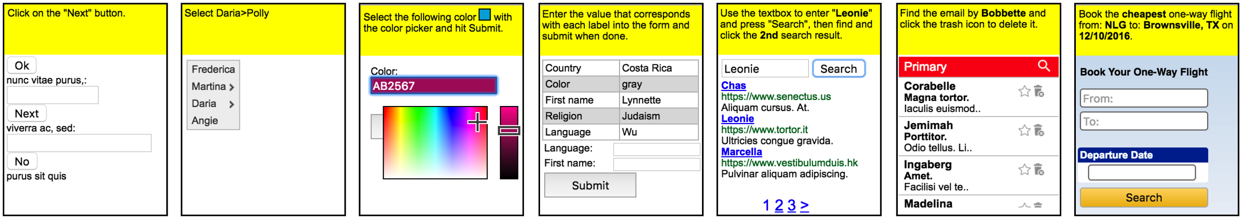
\includegraphics[width=\textwidth, height=\textheight, keepaspectratio]{mwob.png}
	\caption{Example environments from the Mini World of Bits benchmark \cite{mwob}, task prompts are indicated in the yellow section while the white section is the canvas area}
	\label{fig:mwob}
\end{figure*}

Mini World of Bits (MWoB) \cite{mwob} is a new testbed which consists of a wide range of browser-based tasks, such as locating and clicking on an item on the screen, entering text and all the way up to more complex tasks such as searching for a flight between dates. It can be seen as an initial foundation that encapsulates the core functionalities of website interactions, the solving of which would provide strong evidence of development towards performing well on real-world websites. The benchmark is analogous to the MNIST dataset \cite{lecun1998gradient} used in hand-written digit classification in that the ultimate goal for the agents is to be able to perceive and interpret the provided data in a small, self-contained area to complete the task.

We have looked into MWoB due to its novelty: no results have yet been published for this benchmark. By contrast, significant progress has been demonstrated using deep reinforcement learning in other Universe environments such as Atari and Flash games \cite{mnih2013playing}.

\subsection{Hypothesis}
Due to the success of deep reinforcement learning in other experiments, we believe that Deep Q-networks, Vanilla Policy Gradient and Deep Deterministic Policy Gradient algorithms would be effective in MWoB. In perfect information environments, i.e. in tasks whose complete state can be observed from its current visual representation, these models should be able to sufficiently capture the underlying Markov Decision Process. Conversely, in tasks where the agent requires an awareness of past states, models which can capture time dependency, such as Recurrent Neural Networks or Long Short-Term Memory units, would be needed. An example of such an environment within MWoB would be a task where two buttons must be pressed in a particular order, and where no visual feedback is given on whether or not the first button has already been pressed.

\section{Related work}
Various approaches have been used to tackle the RL problem.
The key distinctive feature between these algorithms is whether they aim to explicitly capture the transition dynamics of the environment, or whether they approximate an action policy or an action-value function directly and thus sidestep the problem of uncertainty arising from an unknown environment.
%These can be roughly divided into model-based and model-free methods.
Model-based RL relies on an explicit model of the environment, a Markov Decision Process (MDP), which captures expected rewards of being in each state as well as outgoing transition probabilities from that state given each action. If the model matches the environment, an ideal action policy can easily be sampled from the MDP. Yet, for most interesting problems, the dynamics of the environment are unknown. In this case, a model can be approximated using a deep neural network.

However, the more complicated the environment, the harder it is to learn an accurate representation of it. Perhaps more widespread are model-free RL methods, which, instead of environment dynamics, iterate on either a value function (off-policy learning) \cite{watkins1989learning} or directly on the agent's policy (on-policy learning) \cite{sutton1999policy}.

For any successful RL agent, an important consideration is the balance between exploitation, i.e. extracting the maximum reward out of the environment according to current knowledge, and exploration, in which suboptimal actions are sampled to try to discover new ways to achieve even greater reward. A common strategy is epsilon-greedy \cite{sutton1998reinforcement}, meaning that a random action is chosen with a probability of $\epsilon$, and the remaining actions are greedily sampled from the agent's current approximation. To enable convergence, $\epsilon$ is decayed over time from an initial value of 1 to a near-zero end value.
\subsection{Policy Gradient}
Policy gradient is an on-policy learning algorithm which trains a neural network to create a parametrized stochastic policy $\pi(a|s)$ \cite{sutton1999policy}.
The policy $\pi$ determines a probability distribution over each action $a$ in the action space given a state $s$ of the environment.
The policy is iteratively refined using temporal difference (TD) learning \cite{sutton1988learning} and the network is trained using gradient descent.
During training, rewards received from the environment are used to adjust the policy's parameters such that the probability of actions leading to positive rewards grows and the probability of actions inducing negative rewards is reduced accordingly.
%In the Mini World of Bits benchmark, the goal is to move the cursor to the specified target (button or text box) as close as possible and reward the agent if it manages to hit the button and learn from the chosen action'��s reward. 
%\\In this research, the vanilla Policy Gradient was chosen as the main on-policy approach. To get a basic vanilla Policy Gradient to work, we had to do some visual manipulation to the state and use discrete action spaces with a Convolutional Neural Network (CNN) as the policy. At first, we tried to use a fully connected network as the policy, however the network has too many parameters and is more difficult to train whereas CNN considers neighbouring pixels to shrink down the calculation time and space.

\subsection{Q-learning}
Another notable variant of model-free RL is Q-learning\cite{watkins1989learning}, which approximates an action-value function $Q(S, A)$, representing how much value the agent predicts it will receive in the long run from taking action $A$ in state $S$. For a time step $t$, $Q$ is defined\cite{qlearning} as \[Q(S_t, A_t) = R_t + \gamma Q(S_{t+1}, A_{t+1})\] where $R_t$ is the reward received after taking action $A; S_{t+1}$ the state transitioned to; and $\gamma$ the discount factor [0, 1], which determines the importance of future rewards relative to current ones.  A \(\gamma\) of 0 causes future rewards beyond the current time step to be neglected, whereas a \(\gamma\) of 1 gives a distant future reward equal weight as a reward in the near future. An action is selected by calculating the maximum Q-value of the action space in the current state. In order to eventually converge at an optimal policy, the Q-function is updated by minimising TD error at each time step $t$:
\begin{align*}
Q\left( \mbox{S}_{t},\; A_{t} \right)\; &\leftarrow\;Q\left( \mbox{S}_{t},\; A_{t} \right)\;\\ 
&+\; \alpha_{t}\left[ R_{t+1}\; +\; \gamma \max _{a}Q\left( \mbox{S}_{t+1},\; A \right)\; -\; Q\left( \mbox{S}_{t},\; A_{t} \right) \right]
\end{align*}
\indent
consisting of:
\begin{itemize}
\item \({{\alpha}}_{{t}}\) : The learning rate (or step size). This is initially set to 1 and slowly converges to a value close to 0. This rate determines to what extent is the Q-function still learning and changes to its policy. Once it converges to its designed minimum, the agent will not continue to learn.
\item \(\max _{a}Q\left( \mbox{S}_{t+1},\; A \right)\) : This retrieves the Q-value of the action with the highest value within a set of actions \textit{A} for state \textit{S}
\end{itemize}


Q-learning can converge on an optimal action-selection policy for a discrete MDP, however, policy gradient methods are more suitable to be adapted for continuous action domains.

\subsubsection{Deep Q-learning}
For an environment with discrete states, the Q-function can be implemented as a lookup table. However, the problem with naive Q-learning is that dynamic environments can exhibit a large scope of state-action pairs, and without any form of generalization, iterating through each possible state-action pair is highly impractical. Slight changes to the Q-values also have a tendency to result in significant changes to the policy that can diverge the optimization of the Q-function. This problem was addressed by the Deep Q-network (DQN) proposed by Mnih et al. in 2013 \cite{deepqlearning}. DQNs use deep neural networks as Q-function approximators with weights \(\theta\) to help stabilize convergence.
%serving as the primary architecture of our off-policy implementation.
There are three main components to the Deep Q-network as follows:
\begin{itemize}
\item \textbf{Convolutional Neural Network} : 
The main Q-network is implemented as a Convolutional Neural Network (CNN). This performs feed-forward operations by applying local filter operations on incoming pixels values, performing calculations over a series of convolution layers with a final output of Q-values over a set of actions \(A\). It is this CNN that enables a generalization of state-action pairs in the form of network weights \(\theta\).\linebreak

\item \textbf{Target Network} :
Mnih et al. make use of a secondary neural network that is, for the most part, a duplicate of the Q-Network mentioned above, but with its parameters \(\theta\) copied over with a delay of $n$ steps. The Q-values produced from this network are used to compute the TD loss function. In this way, the delay in updating the target values adds stability to the learning process. For a target network with parameters \(\theta ^{-}\) and a Q-network with parameters \(\theta\), the target value is defined in \cite{deepqlearning} as follows :
\begin{align*}
T_{DQN}\; = ( R\; +\; \lambda \max _{a}Q\left( \mbox{S}_{t+1},\; A_{t+1},\; \theta ^{-} \right)
\end{align*}

With the loss function defined as follows:
\begin{align*}
L\left( \theta  \right)\; =\; \mbox{E}_{\mbox{S},A,\mbox{S}_{t+1},R,D}\; \cdot \; \left[ \left(T_{DQN}\; -\; Q\left( \mbox{S},\; A,\; \theta  \right) \right)^{2}\right]
\end{align*}

\item \textbf{Experience Replay} : Before the training process, the agent's experiences at each time step $t$ are stored in the form of a tuple represented as (\({{S}}_{{t}}\), \({{A}}_{{t}}\), \({{R}}_{{t+1}}\), \({{S}}_{{t+1}}\), \(d\)), with \(d\) a boolean variable signifying if the step completes the episode. These tuples are stored in a replay memory \(D\) with a certain initial capacity. At every training step, the agent samples a batch of tuples from \(D\) that is fed into the network to update the Q-function. This process was later improved upon with the introduction of \textit{Prioritized Experience Replay}\cite{per}, which makes an addition of error-indices to each tuple, representing how much this experience differs from the predictions of the policy, and stores the tuples in a binary heap tree instead of a linear buffer.
\end{itemize}

Both the inclusion of a target network and the randomization of the order of experiences to train on assist with stabilizing the convergence of the Q-values \cite{deepqlearning}. When only a single network is used both for function approximation as well as target value generation or if current experiences are directly used in training, individual trajectories of the agent in the environment are more likely to influence the target values, leading to divergence in the long run.

\subsubsection{Dueling Deep Q-Learning}
Building on the DQN architecture, the Dueling DQN approach \cite{wang2015dueling} splits the single output layer of the CNN into two streams, state-value $V$ and advantage $A$, which are then re-combined to produce the final action-value function $Q(a,s) = V(s) + A(a | s)$. The advantage function $A(a | s)$ quantifies how much better than average it is to take action $a$ given state $s$. The rest of the Reinforcement Learning architecture remains intact.

\subsubsection{Double Deep Q-learning}
The DQN uses a max operator to select and evaluate actions upon a given state with the target network. The problem with this approach is that this can lead to selection of overestimated values, which can delay the time in learning the optimal policy. A simple improvement to this, referred to as the Double Deep Q-Network \cite{doubledeepqlearning}, uses a different equation to update the target value :
\begin{align*}
T_{DDQN}\; =\; R\; +\; \lambda Q\left( \mbox{S}_{t+1},\; \mbox{argmax}Q\left( \mbox{S}_{t+1},\; a,\; \theta ^{-} \right),\; \theta ^{-} \right)
\end{align*}
\subsection{Imitation learning}
In scenarios with large action spaces and complicated tasks, exploring the entire action space uniformly at random can be intractable. In such a case, training can more efficiently begin based on a set of supervised, ideal actions. In Inverse Reinforcement Learning, the agent learns the reward function of the environment by observing these optimal actions performed by an expert, rather than learning a policy or a value function through its own actions. Using this learning method, Abbeel and Ng were able to retrieve a policy with comparable performance to that of the original expert \cite{abbeel2004apprenticeship}.
\section{Methodology}

\subsection{Environments}

\begin{figure}[h!]
	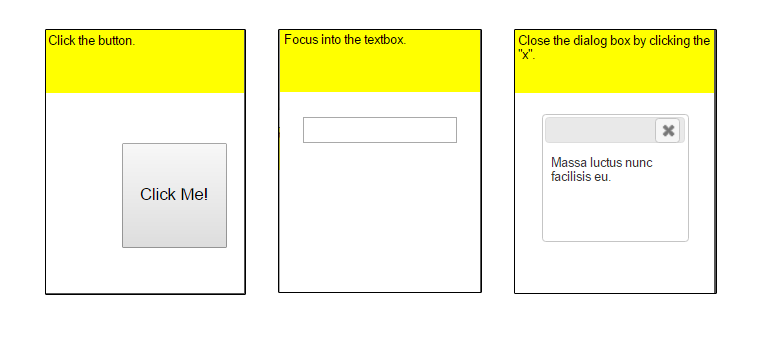
\includegraphics[width=\linewidth]{chosen-envi.png}
	\caption{Environments 1. Click The Button, 2. Focus Into The Textbox, 3. Close The Dialog Box}
	\label{fig:chosen-envi}
\end{figure}

The benchmark consists of 80 environments, which are written in a combination of HTML, JavaScript and CSS, although the agents can not perceive this information via Universe. Each environment is a 210px by 160px webpage, where the yellow section indicates the task prompt and the white section is the canvas area for performing the task (examples of environments can be seen in figure \ref{fig:mwob}). The agents receive visual information in the form of raw pixel values of the webpage and can produce a combination of keyboard or mouse actions while attempting to complete the task. They also receive a reward value based on their performance, ranging 0 to 1 if the task is completed (dependent on the time taken for completion) and -1 if the task is failed or time has run out.

To limit the scope of the problem, we chose a few environments to focus on. There are four categories of environments within WMoB: click tasks, drag tasks, mouse tasks and other tasks. For now, our main goal was to tackle click tasks problems, out of which we left out environments that require Natural Language Processing. In the following sections, we report results on three environments depicted in figure \ref{fig:chosen-envi}: click the button, focus into the textbox, and close the dialog box.

These three environments pose similar tasks that are achievable by creating a policy that clicks on the right area of the 2D action space. Unfortunately, the environments' source code has not yet been released, as MWoB is still in its early stage release. This prevented us from designing new tasks and restricted our use of environments to the ones provided.
%Therefore, the research is solely focusing on training the agents on the available environments using different models and techniques.

\subsection{Action spaces}
An agent performs a series of actions to interact with the environment in hopes of obtaining a reward signal, with the primary objective of maximizing the cumulative reward given the current state of the environment. When we consider the set of actions an agent is allowed to perform, this set can either be \textbf{discrete} or \textbf{continuous}. A discrete action space is simply a fixed set of actions that an agent can perform. Continuous action spaces, on the other hand, are based on one or more continuous dimensions, such as the coordinates on a two-dimensional plane. %Continuous action spaces are more complex, often involving function approximations to determine an approximation of the optimal action for a given state. \linebreak

The Universe platform allows agents to utilize the full set of keyboard presses and mouse controls when defining their action space.
%When we consider the dynamic nature of the environments, this presents a continuous set of state spaces over time.
However, depending on the kind of task an agent is set out to do, we can discretize this vast space to a handful of standard actions that are needed to solve the problem at hand.
When we consider conventional human behavior, controlling \textit{mouse-based} applications often involves the use of moving the cursor in a sequence of directions and clicking upon their target of interest. If we were to discretize this representation for a set of actions for a single frame in time, the cursor would either move in one of four basic directions (up, down, left, right), click on the spot, or do nothing at all. This representation of the action space was our initial starting point for the agent. In this work, we focus on mouse-based tasks only, and omit the use of keyboard presses in order to significantly reduce the dimensionality of the action space and speed up training. %scale down the testing grounds of our agents. %to environments that require completion of tasks using mouse-controls only.
\linebreak

Of course, the above model of the action space does not address many other factors that arise in controlling browser-based applications. For example, we do not consider non-cardinal directions, dragging actions, or scroll actions to navigate through pages to find elements of interest. Furthermore, the discretization of action spaces is a poor solution when it comes to speed. A more efficient solution can easily be defined, namely for the cursor to simply warp to a point on the canvas -- similar to an individual clicking a point on a touchscreen. However, when we consider the scale of the canvas' dimensions of 160x160 pixels (25,600 possible cursor positions), considering each pixel in this space as an individual action would be inefficient and computationally expensive, and thus approximating this space using continuous action spaces is a more efficient solution if we were to consider this approach. Yet realistically, a majority of conventional browser tasks require contextual awareness of the tasks to be performed rather than the actions themselves, which is why our approach first defines the basic foundations of movement and control, which further complexities can be built upon.

\subsection{Input processing}
Generated states for any environment within Universe are represented as raw pixel data, which serve as the primary source of visual context for any agent. As this was the sole means of supervision used in the training process, we sought to investigate techniques to manipulate this data that could help provide an increase in efficiency during training. Some general methods, such as converting images from RGB to grayscale for environments that did not require color co-ordination, and downsampling images to reduce their size, decreased the amount of computation required for an agent to interpret the pixels. In addition, the pixel data was supplemented with more complex additions with the aim of providing increased contextual awareness for the agent.

\begin{figure}[h!]
\centering
	\subfloat{%
	\begin{minipage}[b][8cm][t]{.2\textwidth}
	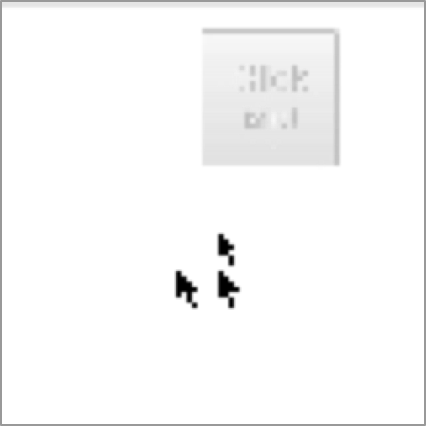
\includegraphics[width=0.9\columnwidth]{downsample.png}
	\vfill
	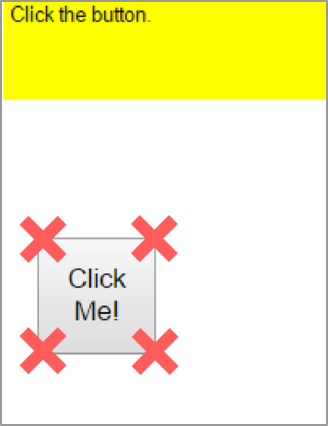
\includegraphics[width=0.9\columnwidth]{edge.png}
	\end{minipage}}
	\subfloat{%
	
\includegraphics[width=1.25in]{fov.png}}\quad
	\caption{Screen shots of different input processing techniques. The top left is a grayscaled and downsampled image of 84x84 pixels. Additionally, the key addition is that the last four frames before the current state are stacked into one image to provide directional information. The right image also uses a downsampled view of the canvas. This method, however, makes use of an additional field-of-view for the agent, or a sort of \textit{"second eyesight"} that has a magnified view of the cursor up-close that also follows its movement. The bottom-left presents an illustration for an implementation of Harris Corner Detection using the SciKit-Image library. This corner data is given to the agent along with the pixel information to identify features (buttons, checkboxes, etc.) on the canvas more easily.}
	\label{fig:inputprocessing}
\end{figure}

Figure \ref{fig:inputprocessing} presents three screen-shots that showcase some of these additions.  All these processing techniques have a general aim of providing an increased sense of supervision to the agent in hopes of speeding up the training process.

\subsection{Implemented models}
One way to train agents on this environment is to use on-policy and off-policy methods. On-policy methods create a policy to make decisions that are improved over time using the agent's action-value function. In off-policy methods such as Q-learning, the agent is using a second greedy policy to determine the value of its actions, regardless of what the current policy recommends \cite{sutton1998reinforcement}. We chose to implement Policy Gradient algorithms (on-policy) as well as Double DQNs and Double Dueling DQNs (off-policy).
\subsubsection{On-policy methods}  
In this work, Vanilla Policy Gradient (PG) was chosen as the main on-policy approach due to its relative simplicity as well as flexibility in the selection of an action space.
On top of that, a theoretical advantage of this approach is that the policy itself does not need to be parametrized, which means that any arbitrary policy can be represented \cite{Peters:2010}.

It proved challenging to fit Vanilla PG into the MWoB environment without any supporting pre-processing. Hence, we added visual manipulation to the input state, such as cropping, converting RGB to greyscale, and corner detection. At first, we used a fully connected network as the policy approximator, but this resulted in the network having too many parameters and being more difficult to train \cite{LongSD14}. To resolve this, the network was replaced with a CNN which considers local neighbourhoods of pixels to shrink down the calculation time and space.

We used TensorFlow to implement the CNN, expand the network with additional layers, train its weights, and process modify. To interface with the MWoB and Gym environments, TensorFlow played a crucial role in simplifying and shaping the agent's input and output. On top of that, TensorFlow came with the advantage of in-built TensorBoard logging to track the agent's performance throughout the training process.

\subsubsection{Off-policy methods}  
An agent following an off-policy approach inherits the behavior of following the recommendation actions off of a second \(\epsilon\)-greedy policy, rather than an action the actual policy \(\pi\) might recommend it to take. This might result an agent to take actions of large consequences, but slowly learns to converge to an optimal policy over time. In this project, we decided to primarily look into adaptations of the Deep Q-network.\linebreak

\paragraph{\bf Deep Q-learning}
Considering the approach we took models a discrete action space, Deep Q-networks were adaptable with this environment. The incorporation of a Convolutional Neural Network (CNN) allowed us to easily feed the pixel data (having been processed with techniques mentioned above) to the network and provide predictions for a fixed number of actions. As described earlier, mouse-based controls were generalized to 5 discrete actions (with also an additional 6th for an agent to do nothing).\linebreak

We did, however, encounter some issues when experimenting with the Experience Replay technique and the hyper-parameters of the agent itself. The MWoB environments have a tendency to produce states with no pixel data at all (only a [None] state) if an episode were to complete when the time elapsed. This is known nature emitted by the environment to the Universe platform and we had to decide how to deal with storing tuples if such transition arises, and if omitting this transition entirely would affect the training process of the network. Another potential improvement we came across was implementing \textit{Prioritized Experience Replay} as explained above. However, calculating error-indices for tuples stored in the binary heap tree relies on positive-only rewards, which renders it infeasible for our environments, which include negative rewards.

Considering that each episode within any MWoB environment includes a time limit and an adjustable frames per second variable, this added to the challenge of identifying optimal initial hyper-parameters of the network that would influence the training process (even to some extent, whether it would train at all). By default, our environment ran at 15 frames per second  -- which puts an upper limit on the frequency of the agent's actions. Within the scope of the 'Click-Test' environment, the worst-case for the number of steps per episode is 150 steps (due to the time constraint set to 10 seconds). This meant that episodes can finish rapidly, and it followed that the target network had to be updated rather quickly in order to avoid the convergence of predicted-values to 0, and a much smaller replay memory size was required for the Experience Replay process.\linebreak

\begin{figure}[h]
\centering
	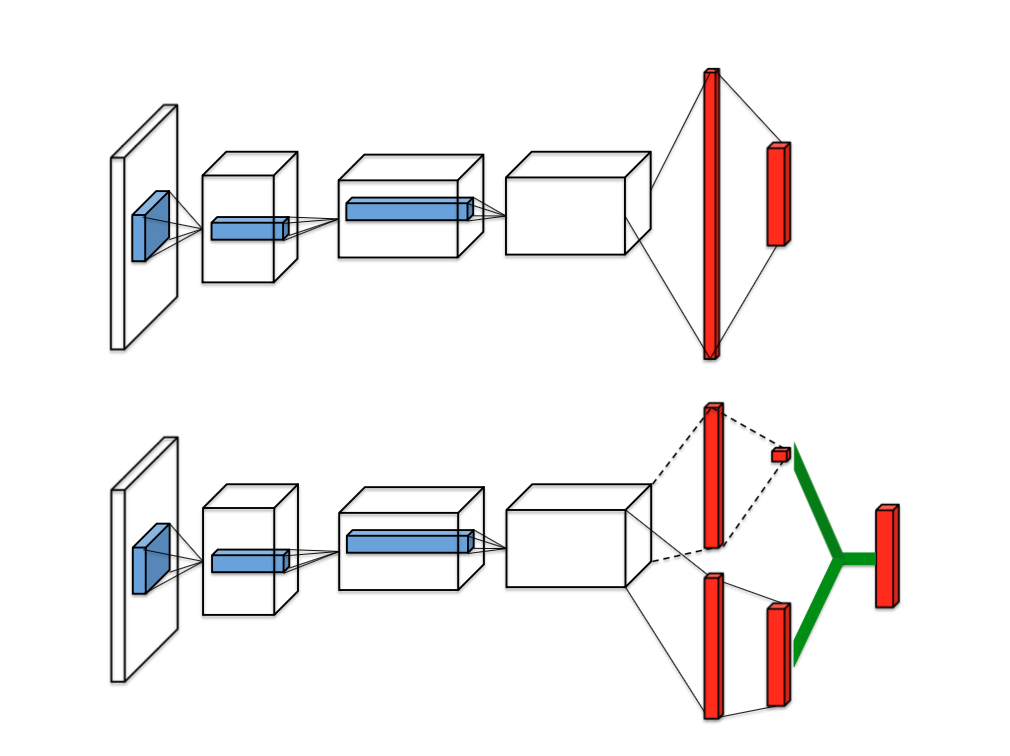
\includegraphics[width=\columnwidth, keepaspectratio]{dueling.png}
	\caption{Illustration comparing the difference between a regular DQN and a Dueling DQN within the neural network}
	\label{fig:dueling}
\end{figure}

\subsection{Reward manipulation}
Another approach we looked into are additional reward manipulation techniques to supplement the existing reward signals in the hope of improving the efficiency of the training process. One caveat to these environments is that during the learning process, there is a possibility for the sequence of actions to result in the cursor moving outside the canvas area onto irrelevant parts of the environment. While we can simply add boundary checking to prevent this behavior from happening, the agent would not directly learn from this restriction due to a lack of error signal of any sort. To counteract this, if the cursor is located at an edge and performs an action that would result in the cursor moving outside the canvas, we experimented with sending out a negative reward signal of -0.5. \linebreak

Inversely, we also tried providing positive reward signals if the cursor performed progressive steps towards completion of the task. For example, one of the environments involved clicking a randomly generated button within the canvas. One technique involved keeping record of the current position of the generated button, and set up a proximity area around the button. If the agent were to perform an action that would result in the position of the cursor to move closer towards the button, it would receive a positive reward signal of +0.1 for every step it did so. \linebreak

\subsection{Supervised methods}
Inspired by Inverse Reinforcement Learning \cite{abbeel2004apprenticeship}, we also investigated approaches to imitation learning. By observing supervised optimal actions, the agent learns the reward function of the environment before learning the optimal policy to optimize for this reward function. While our method of sampling ideal actions was not necessarily scalable to other environments, it gave us evidence on whether the amount of positive episodes was a limiting factor in agent learning performance.

\subsection{Metrics}
To convey a complete picture of learning performance, we ran each agent through a standard evaluation framework to ensure results between environments and training methods were consistent and could be compared with each other. The metrics we chose included actions per episode, percentage of successful episodes, and mean episode reward. The single most telling of these is, of course, mean reward. However, we felt that only looking at the mean reward does not accurately represent how much better the agent is performing if it is to be able to complete the task than if it did not manage to complete it at all within the 10 second time frame. A negative mean reward could, in fact, obscure the fact that as many as two thirds of the episodes were successful, as the relative weight of a late success is much smaller than that of a miss, -1.

\subsection{Training Setup}
The training procedure for these agents was primarily run on a server comprised of an Nvidia TITAN X GPU. We compiled and installed the TensorFlow library from source to take advantage of additional CPU instructions (SSE4.2, AVX2 and FMA), as well as additional GPU capabilities, such as the Nvidia CUDA platform. These optimizations were to ensure we were reaching as much benefit of performance enhancements as possible for added efficiency to training. The results of all our agents were logged and visualized using the in-built TensorBoard to analyze performance of the agents.


\section{Results}

To evaluate our models, we trained them for 3000 episodes on each of the three environments introduced in section 3.1. A typical learning process is depicted in Figure \ref{fig:tboard}. In 3000 episodes, the mean reward rises from around 0 to around 0.4. A large part of the fluctuations in the training process can be attributed to the inherent randomness of the environment, such as the distance from the cursor to the generated button, and the size of said button.  

For comparison, we included an agent which samples each action uniformly at random. For our agents to add value, they would need to outperform said random agent. Tables \ref{results-clicktest}, \ref{results-focustext} and \ref{results-closedialog} demonstrate a performance improvement of up to 10 percent units in the percentage of successful episodes and a mean reward approximately 0.10 higher than the baseline.

\begin{table}[!h]
%% increase table row spacing, adjust to taste
\renewcommand{\arraystretch}{1.3}
% if using array.sty, it might be a good idea to tweak the value of
% \extrarowheight as needed to properly center the text within the cells
\caption{Results on ClickTest-v0}
\label{results-clicktest}
\centering
%% Some packages, such as MDW tools, offer better commands for making tables
%% than the plain LaTeX2e tabular which is used here.
\begin{tabular}{|c||c|c|}
\hline
Agent & Reward & Success rate \% \\
\hline
Random agent & 0.1196 & 67.20\\
\hline
Dueling DQN & &\\
\hline
Double Dueling DQN & 0.2437 & 78.47\\

\hline
Policy Gradient & 0.1511 & 65.30\\
\hline
\end{tabular}
\end{table}

\begin{table}[!h]
%% increase table row spacing, adjust to taste
\renewcommand{\arraystretch}{1.3}
\caption{Results on FocusText-v0}
\label{results-focustext}
\centering
\begin{tabular}{|c||c|c|}
\hline
Agent & Mean reward & Success rate (\%) \\
\hline
Random agent & 0.3375 & 79.88\\
\hline
Dueling DQN & &\\
\hline
Double Dueling DQN & 0.4377 & 82.80 \\
\hline
Policy Gradient &  0.2165 & 70.55\\
\hline
\end{tabular}
\end{table}


\begin{table}[!h]
\renewcommand{\arraystretch}{1.3}
\caption{Results on CloseDialog-v0}
\label{results-closedialog}
\centering
\begin{tabular}{|c||c|c|}
\hline
Agent & Mean Reward & Success rate (\%) \\
\hline
Random agent & -0.6676 & 21.74 \\
\hline
Dueling DQN & &\\
\hline
Double Dueling DQN & -0.0821 & 58.42\\
\hline
Policy Gradient & &\\
\hline
\end{tabular}
\end{table}

\begin{figure}[h!]
\centering
	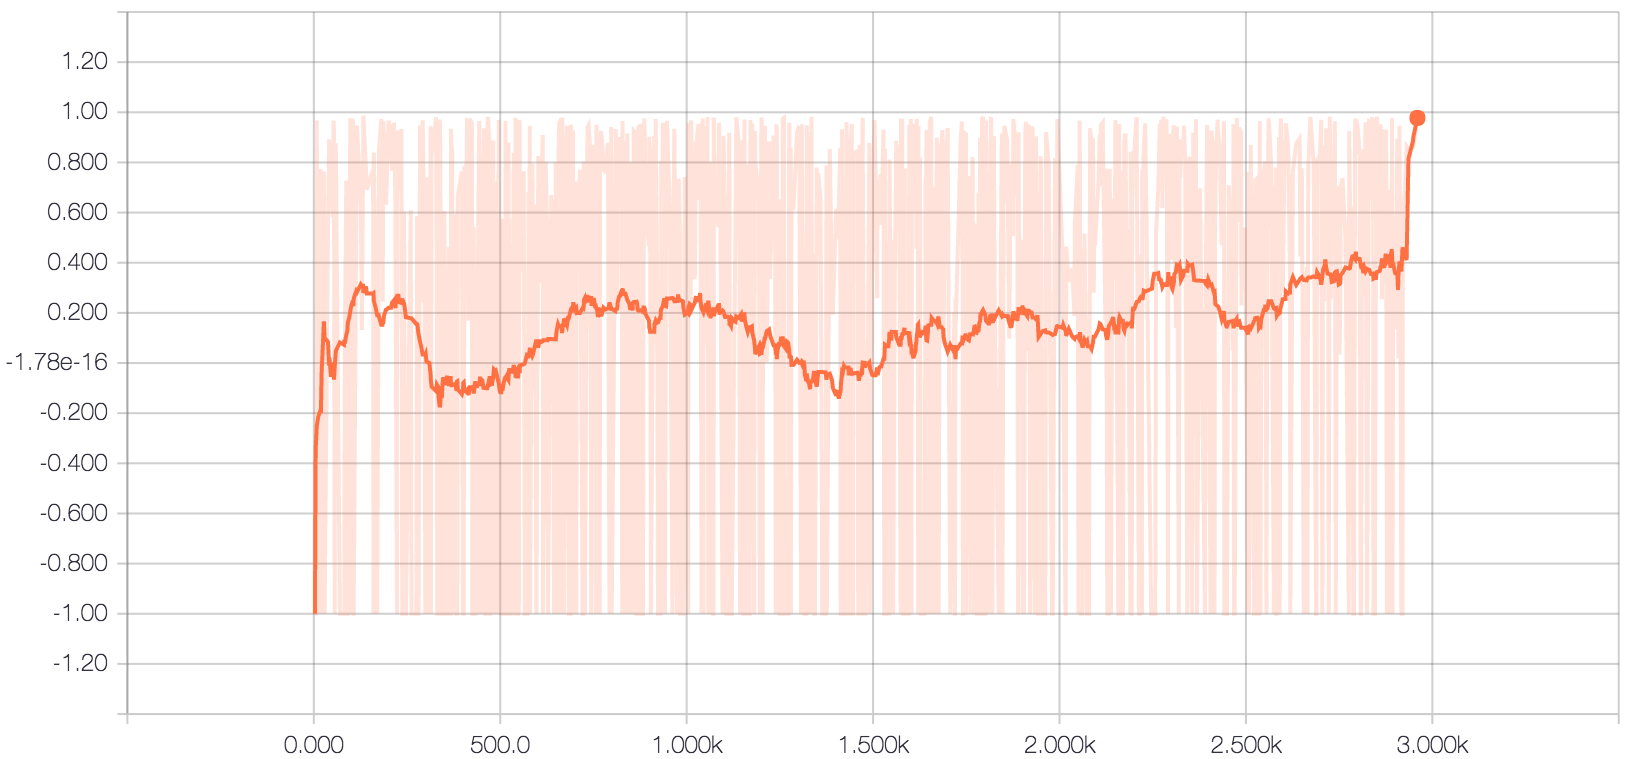
\includegraphics[width=\columnwidth, keepaspectratio]{learningcurve.png}
	\caption{A typical learning curve of our DQN agent on the ClickTest-v0 environment, plotted as reward per episode and smoothed for clarity.}
	\label{fig:tboard}
\end{figure}




\section{Analysis}
%suggestions:
The performance of the baseline random agent also served as an indication of the overall difficulty of the environments.

We also found that including supervised actions to start with did not significantly increase the long-term performance of the agent.

\subsection{Limitations}

\subsubsection{Hardware capability}
Our models combine CNNs with reinforcement learning, providing a good generalisation of methodologies against the clicking tasks. However, it also requires a longer and more intensive training process to train the parameters in the model (the fully connected layers and convolution kernel of the CNN). We are currently training on a machine with only one GPU therefore the training process would hypothetically achieve higher efficiency if a machine (or even a cluster of machines) with multiple GPUs is used instead.

\subsubsection{Lack of environment source code}
Our agent learns under a model-free environment which means limited information access about the environments (only one reward value and image of the section where cursor can move). By taking advantage of source code of the benchmark provided by Dr. Andrej Karpathy later, the agent could be adapted to fully know and interpret certain aspects about the environment, such as what kind of html components there are and their positions/sizes or even the best policy in each step during training process, thus speeding up the training process by using reward manipulation. Also, with the help of a model-based environment, we could analyse the training process by recording and illustrating more criteria (not just the reward value). 

\subsubsection{Runtime errors}
Above this all, there are still some other factors which have affected our training identified within the Universe platform messages, such as the error "reward falling behind"/"throttler fell behind by X seconds" or frame loss.




\section{Conclusion and future work}
\subsection{Conclusion}
Following from the analysis of our results, we can conclude that...
\subsection{Future work}
The novelty of the benchmark indicates still a wide area of progress that can be made, as such there are many future possibilities to expand upon the current state of our project:
\subsubsection{Continuous action spaces}
As we have only discussed discrete action spaces, we would invest more research into implementing continuous action spaces. We are still currently looking into the full implementation and training of an agent via a \textbf{Deep Deterministic Policy Gradient} algorithm \cite{lillicrap2015continuous}, which is specifically designed for continuous action spaces and has shown to be very effective in other non-MWoB environments that use continuous actions, such as the inverted pendulum experiment \cite{pendulum} where the objective is to provide a magnitude to balance the pendulum. The algorithm focuses on an actor-critic method, where the policy function structure is known as the actor, and the value function structure is known as the critic. The actor produces an action given the current state of the environment, and the critic produces a Temporal-Difference error signal given the state and resultant reward. Both the actor and critic learn from the critic's output. In this scenario, neural networks can be used to represent the actor and critic structures, more specifically convolutional neural networks.

We have looked at modelling a magnitude of an action space ranging from -1 to 1 for both angle and distance, where the magnitude is then scaled into a discretised action. This differs to existing solutions which only produce one magnitude for an action. The simple equation below shows how the angle in radians, \( \theta \), is calculated via magnitude \textit{m}:
\[ \theta=m\pi \]
For example, if magnitude was -0.5, the angle to move would be -\( 0.5\pi \). A similar equation would be used to scale the distance \textit{d} by a set fixed distance \textit{D}:
\[ d=mD \]
 Following this, the \textit{x} and \textit{y} distances to move can be calculated accordingly:
 \[ xdist=dsin\theta \]
 \[ ydist=dcos\theta \]
 
This method could prove to be more effective than existing methods that we have implemented due to the fact that hypothetically it would learn quicker; the mouse can navigate to anywhere within the canvas in one step instead of a discretised action space where it would have to slowly navigate to a designated area via several steps.

\subsubsection{Natural language processing}
Another development would be performing natural language processing on the webpage. To elaborate on this with an example, if the question told us to enter a certain word into a text box, we would need NLP to identify this in the prompt in accordance with the agent to correspond with the features identified in the canvas. This can further be extended by analysing the vision to find relevant text via two possible methods:
\indent
\begin{itemize}
\item Optical Character Recognition (OCR) - identify and convert webpage text into machine-encoded text. This is eased by the fact that we are already performing input processing on the image fed to the agent, such that pre-processes in OCR such as binarisation are not needed. 
\item Analysing Document Object Models (DOM) - identify key elements in the webpage where text is concerned. This would further be able to split up certain elements and attempt to classify them for the agent, such as identifying date inputs.
\end{itemize}

\subsubsection{Categorical tasks}
As we have only experimented on environments where clicking an object is the goal of the task, it would be ideal to expand further to other categories of environments, such as dragging and dropping tasks or text-input tasks. Some more complex tasks within the benchmark involve using a combination of these categories e.g drag and drop an object into an area and click submit. It is highly possible that once most, if not all, of the task categories are fulfilled/trained, the agent would be able to train successfully on real-world websites that involve these respective tasks.



% needed in second column of first page if using \IEEEpubid
%\IEEEpubidadjcol



% An example of a floating figure using the graphicx package.
% Note that \label must occur AFTER (or within) \caption.
% For figures, \caption should occur after the \includegraphics.
% Note that IEEEtran v1.7 and later has special internal code that
% is designed to preserve the operation of \label within \caption
% even when the captionsoff option is in effect. However, because
% of issues like this, it may be the safest practice to put all your
% \label just after \caption rather than within \caption{}.
%
% Reminder: the "draftcls" or "draftclsnofoot", not "draft", class
% option should be used if it is desired that the figures are to be
% displayed while in draft mode.
%
%\begin{figure}[!t]
%\centering
%\includegraphics[width=2.5in]{myfigure}
% where an .eps filename suffix will be assumed under latex, 
% and a .pdf suffix will be assumed for pdflatex; or what has been declared
% via \DeclareGraphicsExtensions.
%\caption{Simulation results for the network.}
%\label{fig_sim}
%\end{figure}

% Note that the IEEE typically puts floats only at the top, even when this
% results in a large percentage of a column being occupied by floats.
% However, the Computer Society has been known to put floats at the bottom.


% An example of a double column floating figure using two subfigures.
% (The subfig.sty package must be loaded for this to work.)
% The subfigure \label commands are set within each subfloat command,
% and the \label for the overall figure must come after \caption.
% \hfil is used as a separator to get equal spacing.
% Watch out that the combined width of all the subfigures on a 
% line do not exceed the text width or a line break will occur.
%
%\begin{figure*}[!t]
%\centering
%\subfloat[Case I]{\includegraphics[width=2.5in]{box}%
%\label{fig_first_case}}
%\hfil
%\subfloat[Case II]{\includegraphics[width=2.5in]{box}%
%\label{fig_second_case}}
%\caption{Simulation results for the network.}
%\label{fig_sim}
%\end{figure*}
%
% Note that often IEEE papers with subfigures do not employ subfigure
% captions (using the optional argument to \subfloat[]), but instead will
% reference/describe all of them (a), (b), etc., within the main caption.
% Be aware that for subfig.sty to generate the (a), (b), etc., subfigure
% labels, the optional argument to \subfloat must be present. If a
% subcaption is not desired, just leave its contents blank,
% e.g., \subfloat[].


% An example of a floating table. Note that, for IEEE style tables, the
% \caption command should come BEFORE the table and, given that table
% captions serve much like titles, are usually capitalized except for words
% such as a, an, and, as, at, but, by, for, in, nor, of, on, or, the, to
% and up, which are usually not capitalized unless they are the first or
% last word of the caption. Table text will default to \footnotesize as
% the IEEE normally uses this smaller font for tables.
% The \label must come after \caption as always.
%
%\begin{table}[!t]
%% increase table row spacing, adjust to taste
%\renewcommand{\arraystretch}{1.3}
% if using array.sty, it might be a good idea to tweak the value of
% \extrarowheight as needed to properly center the text within the cells
%\caption{An Example of a Table}
%\label{table_example}
%\centering
%% Some packages, such as MDW tools, offer better commands for making tables
%% than the plain LaTeX2e tabular which is used here.
%\begin{tabular}{|c||c|}
%\hline
%One & Two\\
%\hline
%Three & Four\\
%\hline
%\end{tabular}
%\end{table}


% Note that the IEEE does not put floats in the very first column
% - or typically anywhere on the first page for that matter. Also,
% in-text middle ("here") positioning is typically not used, but it
% is allowed and encouraged for Computer Society conferences (but
% not Computer Society journals). Most IEEE journals/conferences use
% top floats exclusively. 
% Note that, LaTeX2e, unlike IEEE journals/conferences, places
% footnotes above bottom floats. This can be corrected via the
% \fnbelowfloat command of the stfloats package.






% if have a single appendix:
%\appendix[Proof of the Zonklar Equations]
% or
%\appendix  % for no appendix heading
% do not use \section anymore after \appendix, only \section*
% is possibly needed

% use appendices with more than one appendix
% then use \section to start each appendix
% you must declare a \section before using any
% \subsection or using \label (\appendices by itself
% starts a section numbered zero.)
%


%\appendices
%\section{Proof of the First Zonklar Equation}
%Appendix one text goes here.

% you can choose not to have a title for an appendix
% if you want by leaving the argument blank
%\section{}
%Appendix two text goes here.


% use section* for acknowledgment
\ifCLASSOPTIONcompsoc
  % The Computer Society usually uses the plural form
%  \section*{Acknowledgments}
\else
  % regular IEEE prefers the singular form
%  \section*{Acknowledgment}
\fi


%The authors would like to thank...


% Can use something like this to put references on a page
% by themselves when using endfloat and the captionsoff option.
\ifCLASSOPTIONcaptionsoff
  \newpage
\fi



% trigger a \newpage just before the given reference
% number - used to balance the columns on the last page
% adjust value as needed - may need to be readjusted if
% the document is modified later
%\IEEEtriggeratref{8}
% The "triggered" command can be changed if desired:
%\IEEEtriggercmd{\enlargethispage{-5in}}

% references section

% can use a bibliography generated by BibTeX as a .bbl file
% BibTeX documentation can be easily obtained at:
% http://mirror.ctan.org/biblio/bibtex/contrib/doc/
% The IEEEtran BibTeX style support page is at:
% http://www.michaelshell.org/tex/ieeetran/bibtex/
%\bibliographystyle{IEEEtran}
% argument is your BibTeX string definitions and bibliography database(s)
%\bibliography{IEEEabrv,../bib/paper}
%
% <OR> manually copy in the resultant .bbl file
% set second argument of \begin to the number of references
% (used to reserve space for the reference number labels box)
\bibliography{references}
\bibliographystyle{IEEEtran}

%\begin{thebibliography}{1}

%\bibitem{IEEEhowto:kopka}
%H.~Kopka and P.~W. Daly, \emph{A Guide to {\LaTeX}}, 3rd~ed.\hskip 1em plus
%  0.5em minus 0.4em\relax Harlow, England: Addison-Wesley, 1999.

%\end{thebibliography}

% biography section
% 
% If you have an EPS/PDF photo (graphicx package needed) extra braces are
% needed around the contents of the optional argument to biography to prevent
% the LaTeX parser from getting confused when it sees the complicated
% \includegraphics command within an optional argument. (You could create
% your own custom macro containing the \includegraphics command to make things
% simpler here.)
%\begin{IEEEbiography}[{\includegraphics[width=1in,height=1.25in,clip,keepaspectratio]{mshell}}]{Michael Shell}
% or if you just want to reserve a space for a photo:

% You can push biographies down or up by placing
% a \vfill before or after them. The appropriate
% use of \vfill depends on what kind of text is
% on the last page and whether or not the columns
% are being equalized.

%\vfill

% Can be used to pull up biographies so that the bottom of the last one
% is flush with the other column.
%\enlargethispage{-5in}



% that's all folks
\end{document}


